\documentclass[10pt,aspectratio=169]{beamer}

\usetheme{Madrid}
\usecolortheme{default}
\usepackage{amsmath,amssymb,booktabs,array,multirow}
\usepackage{tikz}
\usepackage{pgfplots}
\pgfplotsset{compat=1.18}

\definecolor{hkustblue}{RGB}{0,56,116}
\definecolor{hkustgold}{RGB}{166,124,0}
\setbeamercolor{structure}{fg=hkustblue}
\setbeamercolor{frametitle}{fg=white,bg=hkustblue}
\setbeamercolor{title}{fg=white,bg=hkustblue}
\setbeamercolor{block title}{fg=white,bg=hkustblue}
\setbeamercolor{block body}{bg=blue!3}
\setbeamertemplate{navigation symbols}{}
\setbeamertemplate{footline}[frame number]

\newcommand{\pay}[2]{#1,\ #2}
\newcommand{\br}{\text{BR}}

\title[Game Theory Tutorial]{Tutorial: Introduction to Game Theory (1/2)}
\subtitle{IEDA 1250 Optimizing Decisions for Personal and Business Development}
\author{Wu Hongfan}
\institute{The Hong Kong University of Science and Technology}
\date{June 26, 2026}

\begin{document}

\begin{frame}
  \titlepage
\end{frame}

\begin{frame}{Plan for Today}
\begin{enumerate}
  \item Translate a story into players, strategies, and payoffs.
  \item Find Nash equilibria by best responses and dominated strategies.
  \item Solve zero-sum games with saddle points and mixed strategies.
  \item Connect the method to homework-style questions.
\end{enumerate}
\vspace{0.4cm}
\begin{block}{Target}
By the end, you should be able to read a payoff table and decide which solution method to try first.
\end{block}
\end{frame}

\begin{frame}{What Makes a Situation a Game?}
\begin{block}{A game}
A decision situation where each player's payoff depends on the actions of more than one decision maker.
\end{block}
\vspace{0.2cm}
\begin{columns}[T]
\column{0.48\textwidth}
\textbf{Ingredients}
\begin{itemize}
  \item Players
  \item Strategies
  \item Payoffs
  \item Information and timing
\end{itemize}
\column{0.48\textwidth}
\textbf{Typical assumptions}
\begin{itemize}
  \item Rationality
  \item Self-interest
  \item Common knowledge of the game
  \item Simultaneous or sequential moves
\end{itemize}
\end{columns}
\end{frame}

\begin{frame}{Example: Prisoner's Dilemma}
\begin{center}
\begin{tabular}{c c c c}
 & & \multicolumn{2}{c}{Prisoner B}\\
 & & Silent & Betray\\
\cmidrule{3-4}
\multirow{2}{*}{Prisoner A} & Silent & $\pay{-2}{-2}$ & $\pay{-10}{0}$\\
 & Betray & $\pay{0}{-10}$ & $\pay{-5}{-5}$\\
\end{tabular}
\end{center}
\vspace{0.3cm}
\begin{itemize}
  \item Payoffs are utilities, so fewer years in prison means a larger payoff.
  \item Each player chooses without observing the other player's choice.
  \item The social outcome $(\text{Silent}, \text{Silent})$ is better for both, but it is not stable.
\end{itemize}
\end{frame}

\begin{frame}{Best Response Thinking}
\begin{block}{Best response}
A strategy is a best response if it gives the highest payoff given the other player's strategy.
\end{block}
\vspace{0.2cm}
\begin{center}
\begin{tabular}{c c c c}
 & & \multicolumn{2}{c}{Prisoner B}\\
 & & Silent & Betray\\
\cmidrule{3-4}
\multirow{2}{*}{Prisoner A} & Silent & $\pay{-2}{-2}$ & $\pay{-10}{0}$\\
 & Betray & $\pay{0}{-10}$ & $\pay{-5}{-5}$\\
\end{tabular}
\end{center}
\vspace{0.2cm}
\begin{itemize}
  \item If B is silent, A prefers Betray: $0>-2$.
  \item If B betrays, A prefers Betray: $-5>-10$.
  \item By symmetry, B also prefers Betray in both cases.
\end{itemize}
\end{frame}

\begin{frame}{Nash Equilibrium}
\begin{block}{Nash equilibrium}
A strategy profile where no single player can improve by changing only their own strategy.
\end{block}
\vspace{0.2cm}
\begin{itemize}
  \item ``I am doing my best given what you do.''
  \item ``You are doing your best given what I do.''
  \item It is a stability concept, not necessarily a fairness or efficiency concept.
\end{itemize}
\vspace{0.3cm}
\begin{block}{Prisoner's Dilemma}
The Nash equilibrium is $(\text{Betray}, \text{Betray})$.
\end{block}
\end{frame}

\begin{frame}{How to Read a Payoff Matrix}
\begin{columns}[T]
\column{0.52\textwidth}
\begin{center}
\begin{tabular}{c c c c}
 & & \multicolumn{2}{c}{Column player}\\
 & & L & R\\
\cmidrule{3-4}
\multirow{2}{*}{Row player} & U & $\pay{3}{2}$ & $\pay{0}{3}$\\
 & D & $\pay{2}{1}$ & $\pay{1}{0}$\\
\end{tabular}
\end{center}
\column{0.45\textwidth}
\begin{itemize}
  \item First number: row player's payoff.
  \item Second number: column player's payoff.
  \item Row player chooses a row.
  \item Column player chooses a column.
\end{itemize}
\end{columns}
\vspace{0.25cm}
\begin{block}{Check}
Never compare payoffs across different players. Compare a player's own payoffs while holding the other player's action fixed.
\end{block}
\end{frame}

\begin{frame}{Dominated Strategies}
\begin{block}{Dominated strategy}
Strategy $s$ is dominated if another strategy is always at least as good and sometimes strictly better, regardless of the opponent's action.
\end{block}
\vspace{0.2cm}
\begin{itemize}
  \item For a row player who maximizes: larger row payoffs are better.
  \item For a column player in a zero-sum payoff table for Player 1: smaller entries are better.
  \item Eliminating dominated strategies can simplify a game before solving it.
\end{itemize}
\end{frame}

\begin{frame}{Exercise 1: Eliminate Dominated Strategies}
\begin{center}
\begin{tabular}{c c c c c c}
 & \multicolumn{5}{c}{Player 2}\\
Player 1 & S1 & S2 & S3 & S4 & S5\\
\midrule
S1 & 3 & 2 & 0 & 3 & 0\\
S2 & 5 & 0 & 2 & 5 & 9\\
S3 & 7 & 3 & 9 & 5 & 9\\
S4 & 4 & 6 & 8 & 7 & 5.5\\
S5 & 6 & 0 & 8 & 8 & 3\\
\end{tabular}
\end{center}
\vspace{0.2cm}
\begin{block}{Task}
Assume the entries are payoffs to Player 1. Which strategies can we remove first?
\end{block}
\end{frame}

\begin{frame}{Exercise 1: One Elimination Order}
\begin{enumerate}
  \item Column S4 is dominated by Column S2, so remove Column S4.
  \item Row S1 is dominated by Row S3, so remove Row S1.
  \item Row S2 is dominated by Row S3, so remove Row S2.
  \item In the reduced table, Row S5 is dominated by Row S3, so remove Row S5.
  \item In the reduced table, Column S3 is dominated by Column S5, so remove Column S3.
\end{enumerate}
\vspace{0.2cm}
\begin{block}{Takeaway}
Dominance is a simplification tool. The order may differ, but every removal must be justified by comparing all remaining entries.
\end{block}
\end{frame}

\begin{frame}{Zero-Sum Games}
\begin{block}{Zero-sum game}
One player's gain is exactly the other player's loss.
\end{block}
\vspace{0.2cm}
\begin{itemize}
  \item A single payoff table is enough: entries are payoffs to Player A.
  \item Player A wants to maximize the payoff.
  \item Player B wants to minimize Player A's payoff.
\end{itemize}
\vspace{0.2cm}
\begin{block}{Value of the game}
The expected payoff to Player A when both players use optimal strategies.
\end{block}
\end{frame}

\begin{frame}{Pure Strategy: Saddle Point Test}
\begin{center}
\begin{tabular}{c c c c c c}
 & B1 & B2 & B3 & B4 & Row min\\
\midrule
A1 & 20 & 15 & 12 & 35 & 12\\
A2 & 25 & 14 & 8 & 10 & 8\\
A3 & 40 & 2 & 10 & 5 & 2\\
A4 & -5 & 4 & 11 & 0 & -5\\
\midrule
Col max & 40 & 15 & 12 & 35 & \\
\end{tabular}
\end{center}
\vspace{0.2cm}
\begin{itemize}
  \item Player A chooses the row with largest row minimum: $\max \min = 12$.
  \item Player B chooses the column with smallest column maximum: $\min \max = 12$.
  \item Since they are equal, there is a saddle point.
\end{itemize}
\end{frame}

\begin{frame}{Pure Strategy: Result}
\begin{block}{Saddle point}
The saddle point is $(A1,B3)$ and the value of the game is $12$.
\end{block}
\vspace{0.2cm}
\begin{itemize}
  \item It is the minimum in Row A1.
  \item It is the maximum in Column B3.
  \item If A announces A1, B cannot reduce A below 12.
  \item If B announces B3, A cannot increase above 12.
\end{itemize}
\end{frame}

\begin{frame}{When There Is No Saddle Point}
\begin{center}
\begin{tabular}{c c c c c}
 & B1 & B2 & B3 & Row min\\
\midrule
A1 & 0 & -2 & 2 & -2\\
A2 & 5 & 4 & -3 & -3\\
A3 & 2 & 3 & -4 & -4\\
\midrule
Col max & 5 & 4 & 2 & \\
\end{tabular}
\end{center}
\vspace{0.2cm}
\begin{itemize}
  \item $\max \min = -2$.
  \item $\min \max = 2$.
  \item They are not equal, so no pure strategy saddle point exists.
  \item We need mixed strategies.
\end{itemize}
\end{frame}

\begin{frame}{Mixed Strategies}
\begin{block}{Mixed strategy}
A probability distribution over pure strategies.
\end{block}
\vspace{0.2cm}
\begin{itemize}
  \item Player A may choose A1 with probability $p$ and A2 with probability $1-p$.
  \item Player B may choose B1 with probability $q$ and B2 with probability $1-q$.
  \item The payoff becomes an expected payoff.
\end{itemize}
\vspace{0.2cm}
\begin{block}{Key idea}
At equilibrium, a player randomizes only among strategies that give the same expected payoff.
\end{block}
\end{frame}

\begin{frame}{Graphical Method: Setup}
Use the problem set example:
\begin{center}
\begin{tabular}{c c c c c}
 & B1 & B2 & B3 & B4\\
\midrule
A1 & 2 & 2 & 3 & -2\\
A2 & 4 & 3 & 2 & 6\\
\end{tabular}
\end{center}
\vspace{0.2cm}
Let $p=\Pr(A1)$ and $1-p=\Pr(A2)$. Expected payoffs to A:
\begin{align*}
f_{B1}(p)&=2p+4(1-p)=4-2p,\\
f_{B2}(p)&=2p+3(1-p)=3-p,\\
f_{B3}(p)&=3p+2(1-p)=2+p,\\
f_{B4}(p)&=-2p+6(1-p)=6-8p.
\end{align*}
\end{frame}

\begin{frame}{Graphical Method: Maximize the Lower Envelope}
\begin{center}
\begin{tikzpicture}
\begin{axis}[
  width=0.78\textwidth,height=0.55\textheight,
  xmin=0,xmax=1,ymin=-2,ymax=7,
  xlabel={$p=\Pr(A1)$},ylabel={Expected payoff to A},
  legend pos=north east,grid=major]
\addplot[blue,thick,domain=0:1]{4-2*x}; \addlegendentry{$B1$}
\addplot[teal,thick,domain=0:1]{3-x}; \addlegendentry{$B2$}
\addplot[orange,thick,domain=0:1]{2+x}; \addlegendentry{$B3$}
\addplot[red,thick,domain=0:1]{6-8*x}; \addlegendentry{$B4$}
\addplot[black,only marks,mark=*] coordinates {(4/9,22/9)};
\node at (axis cs:0.49,2.85) {$p=4/9,\ V=22/9$};
\end{axis}
\end{tikzpicture}
\end{center}
\vspace{-0.2cm}
\begin{block}{Result for Player A}
Choose $(A1,A2)=\left(\frac{4}{9},\frac{5}{9}\right)$ and guarantee value $V=\frac{22}{9}$.
\end{block}
\end{frame}

\begin{frame}{Why the Intersection Matters}
\begin{itemize}
  \item Player B chooses the column that gives A the smallest expected payoff.
  \item So A cares about the minimum of the four lines.
  \item A chooses $p$ to make this minimum as large as possible.
  \item The best point occurs where the binding lines $B3$ and $B4$ meet:
\end{itemize}
\[
2+p=6-8p \quad \Rightarrow \quad p=\frac{4}{9}.
\]
\[
V=2+\frac{4}{9}=\frac{22}{9}.
\]
\end{frame}

\begin{frame}{Check the Binding Lines}
At $p=4/9$:
\begin{align*}
f_{B1}(4/9)&=4-8/9=28/9,\\
f_{B2}(4/9)&=3-4/9=23/9,\\
f_{B3}(4/9)&=2+4/9=22/9,\\
f_{B4}(4/9)&=6-32/9=22/9.
\end{align*}
\vspace{0.2cm}
\begin{block}{Binding constraints}
The binding columns are $B3$ and $B4$, so Player B places positive probability only on $B3$ and $B4$.
\end{block}
\end{frame}

\begin{frame}{Find Player B's Mixed Strategy}
Let $q_j=\Pr(Bj)$. Since $B3$ and $B4$ are binding, try
\[
q_1=q_2=0,\quad q_3+q_4=1.
\]
Make A indifferent between A1 and A2:
\[
3q_3-2q_4 = 2q_3+6q_4.
\]
\[
q_3=8q_4,\quad q_3+q_4=1.
\]
\begin{block}{Result for Player B}
\[
(B1,B2,B3,B4)=\left(0,0,\frac{8}{9},\frac{1}{9}\right).
\]
\end{block}
\end{frame}

\begin{frame}{Graphical Method Checklist}
\begin{enumerate}
  \item If Player A has two rows, let $p$ be the probability of the first row.
  \item Write one expected payoff line for each column of Player B.
  \item Draw or compare the lower envelope.
  \item Choose the $p$ that maximizes the lower envelope.
  \item Binding columns get positive probability for Player B.
  \item Use indifference equations to find Player B's probabilities.
\end{enumerate}
\end{frame}

\begin{frame}{Practice 2: A 6-by-2 Graphical Problem}
\begin{center}
\begin{tabular}{c c c}
 & B1 & B2\\
\midrule
A1 & 1 & -3\\
A2 & 3 & 5\\
A3 & -1 & 6\\
A4 & 4 & 1\\
A5 & 2 & 2\\
A6 & -5 & 0\\
\end{tabular}
\end{center}
\vspace{0.2cm}
\begin{block}{Task}
This time Player B has two columns. Let $q=\Pr(B1)$. Which row payoff lines should determine the solution?
\end{block}
\end{frame}

\begin{frame}{Practice 2: Payoff Lines}
\[
\begin{aligned}
g_{A1}(q)&=1q-3(1-q)=-3+4q,\\
g_{A2}(q)&=3q+5(1-q)=5-2q,\\
g_{A3}(q)&=-q+6(1-q)=6-7q,\\
g_{A4}(q)&=4q+1(1-q)=1+3q,\\
g_{A5}(q)&=2,\\
g_{A6}(q)&=-5q.
\end{aligned}
\]
\vspace{0.2cm}
\begin{block}{Player B's goal}
Player B chooses $q$ to minimize the upper envelope, because A will choose the best row after seeing expected payoffs.
\end{block}
\end{frame}

\begin{frame}{Practice 2: Result}
The solution is determined by rows A2 and A4:
\[
5-2q = 1+3q \quad \Rightarrow \quad q=\frac{4}{5}.
\]
\[
V=5-2\cdot\frac{4}{5}=\frac{17}{5}=3.4.
\]
To find A's probabilities, let A mix A2 with probability $p$ and A4 with probability $1-p$:
\[
3p+4(1-p)=5p+1(1-p).
\]
\[
4-p=1+4p \Rightarrow p=\frac{3}{5}.
\]
\begin{block}{Optimal strategies}
A: $(0,\frac{3}{5},0,\frac{2}{5},0,0)$, \quad B: $(\frac{4}{5},\frac{1}{5})$.
\end{block}
\end{frame}

\begin{frame}{LP Formulation for Zero-Sum Games}
For Player A with mixed strategy $x_i$ and game value $V$:
\[
\max V
\]
\[
\sum_i a_{ij}x_i \ge V \quad \text{for every column } j
\]
\[
\sum_i x_i=1,\quad x_i\ge 0.
\]
\vspace{0.2cm}
\begin{itemize}
  \item Each column constraint says: if B chooses this column, A's expected payoff is at least $V$.
  \item Maximize the guaranteed payoff.
  \item This is another way to express the minimax idea.
\end{itemize}
\end{frame}

\begin{frame}{From Zero-Sum to Business Competition}
\begin{itemize}
  \item Not all games are zero-sum.
  \item In business, firms may both earn positive profits.
  \item The Nash equilibrium idea still applies: each firm chooses a best response to the other.
\end{itemize}
\vspace{0.2cm}
\begin{block}{Cournot competition}
Firms choose quantities simultaneously. The market price depends on total quantity.
\end{block}
\end{frame}

\begin{frame}{Cournot Model}
Two firms choose $q_1$ and $q_2$.
\[
p=a-b(q_1+q_2)
\]
If both firms have unit cost $c$, firm 1's profit is
\[
\pi_1=[a-b(q_1+q_2)-c]q_1.
\]
Firm 1's best response:
\[
q_1^*=\frac{a-c-bq_2}{2b}.
\]
Similarly,
\[
q_2^*=\frac{a-c-bq_1}{2b}.
\]
\end{frame}

\begin{frame}{Cournot Equilibrium}
Solve the two best-response equations:
\[
q_1^*=\frac{a-c-bq_2}{2b},\qquad
q_2^*=\frac{a-c-bq_1}{2b}.
\]
For symmetric firms:
\[
q_1^*=q_2^*=\frac{a-c}{3b}.
\]
\vspace{0.2cm}
\begin{block}{Interpretation}
Each firm produces less than the perfectly competitive level, because each firm knows that more output lowers the market price.
\end{block}
\end{frame}

\begin{frame}{Cournot Practice}
\begin{block}{Problem}
Market price is $p=14-2Q$, where $Q=q_1+q_2$. Firm 1 has unit cost 2 and Firm 2 has unit cost 4. Find the equilibrium quantities.
\end{block}
\vspace{0.2cm}
\[
\pi_1=(14-2q_1-2q_2-2)q_1=(12-2q_1-2q_2)q_1.
\]
\[
\pi_2=(14-2q_1-2q_2-4)q_2=(10-2q_1-2q_2)q_2.
\]
\end{frame}

\begin{frame}{Cournot Practice: Solution}
First-order conditions:
\[
\frac{\partial \pi_1}{\partial q_1}=12-4q_1-2q_2=0
\Rightarrow q_1=3-\frac{1}{2}q_2.
\]
\[
\frac{\partial \pi_2}{\partial q_2}=10-2q_1-4q_2=0
\Rightarrow q_2=2.5-\frac{1}{2}q_1.
\]
Solve:
\[
q_1^*=\frac{7}{3},\qquad q_2^*=\frac{4}{3}.
\]
\end{frame}

\begin{frame}{Which Method Should I Use?}
\begin{center}
\begin{tabular}{p{0.36\textwidth} p{0.46\textwidth}}
\toprule
Situation & Good first method\\
\midrule
Obvious bad rows or columns & Dominated strategy elimination\\
Zero-sum table, pure solution possible & Saddle point test\\
Two rows or two columns, no saddle point & Graphical mixed strategy method\\
Larger zero-sum game & LP formulation\\
Business competition with continuous decisions & Best-response functions\\
\bottomrule
\end{tabular}
\end{center}
\end{frame}

\begin{frame}{Common Mistakes}
\begin{itemize}
  \item Comparing Player A's payoff with Player B's payoff in the same cell.
  \item Forgetting that Player B minimizes A's payoff in a zero-sum table.
  \item Declaring a Nash equilibrium without checking unilateral deviations.
  \item In graphical method, using the wrong envelope: lower envelope for A's two-row problem, upper envelope for B's two-column problem.
  \item Forgetting probabilities must sum to one and be nonnegative.
\end{itemize}
\end{frame}

\begin{frame}{Mini Quiz}
\begin{enumerate}
  \item In a Nash equilibrium, can the outcome be inefficient?
  \item In a zero-sum game, what does Player B want to do to Player A's payoff?
  \item What equality must hold for a saddle point?
  \item If Player A mixes between two rows, what must be true about the expected payoff of those two rows?
\end{enumerate}
\end{frame}

\begin{frame}{Summary}
\begin{itemize}
  \item Game theory studies decisions where payoffs depend on other decision makers.
  \item Nash equilibrium is a no-unilateral-deviation condition.
  \item Dominance and saddle point tests are fast first checks.
  \item Mixed strategies use probabilities to create stable expected payoffs.
  \item Graphical and LP methods are practical tools for zero-sum games.
\end{itemize}
\vspace{0.3cm}
\begin{block}{For homework}
Start each problem by identifying the game type and the solution method before doing algebra.
\end{block}
\end{frame}

\begin{frame}{References Used in Preparation}
\small
\begin{itemize}
  \item IEDA 1250 Lecture 4: Introduction to Game Theory, Prof. Bo Yang, Summer 2026.
  \item IEDA 1250 Game Theory problem set and lecture exercises, Summer 2026.
  \item UCSD undergraduate game theory slides, V. Crawford.
  \item Bonanno, \emph{Game Theory}, 3rd edition.
  \item Brown CS lecture slides on introductory game theory.
\end{itemize}
\end{frame}

\end{document}
